\chapter{Integration tests}

This integrations test is focusing on the integration between hardware and software, since hardware integration is explained in section~\ref{sec:hardware_int} on page~\pageref{sec:hardware_int} and software integration is explained in section~\ref{sec:software_int} on page~\pageref{sec:software_int}. 

To complete the integration test, all that need to be done is for the software to be put on the the Raspberry pi. When it's on there it need to get compiled. And if all of the components are connected as it should be, the testing can continue. 

In figure~\ref{fig:integration_setup}, the setup used for the integration test can be seen. When the boat should move it should just be picked up and actually moved.

\begin{figure}[H]
\centering
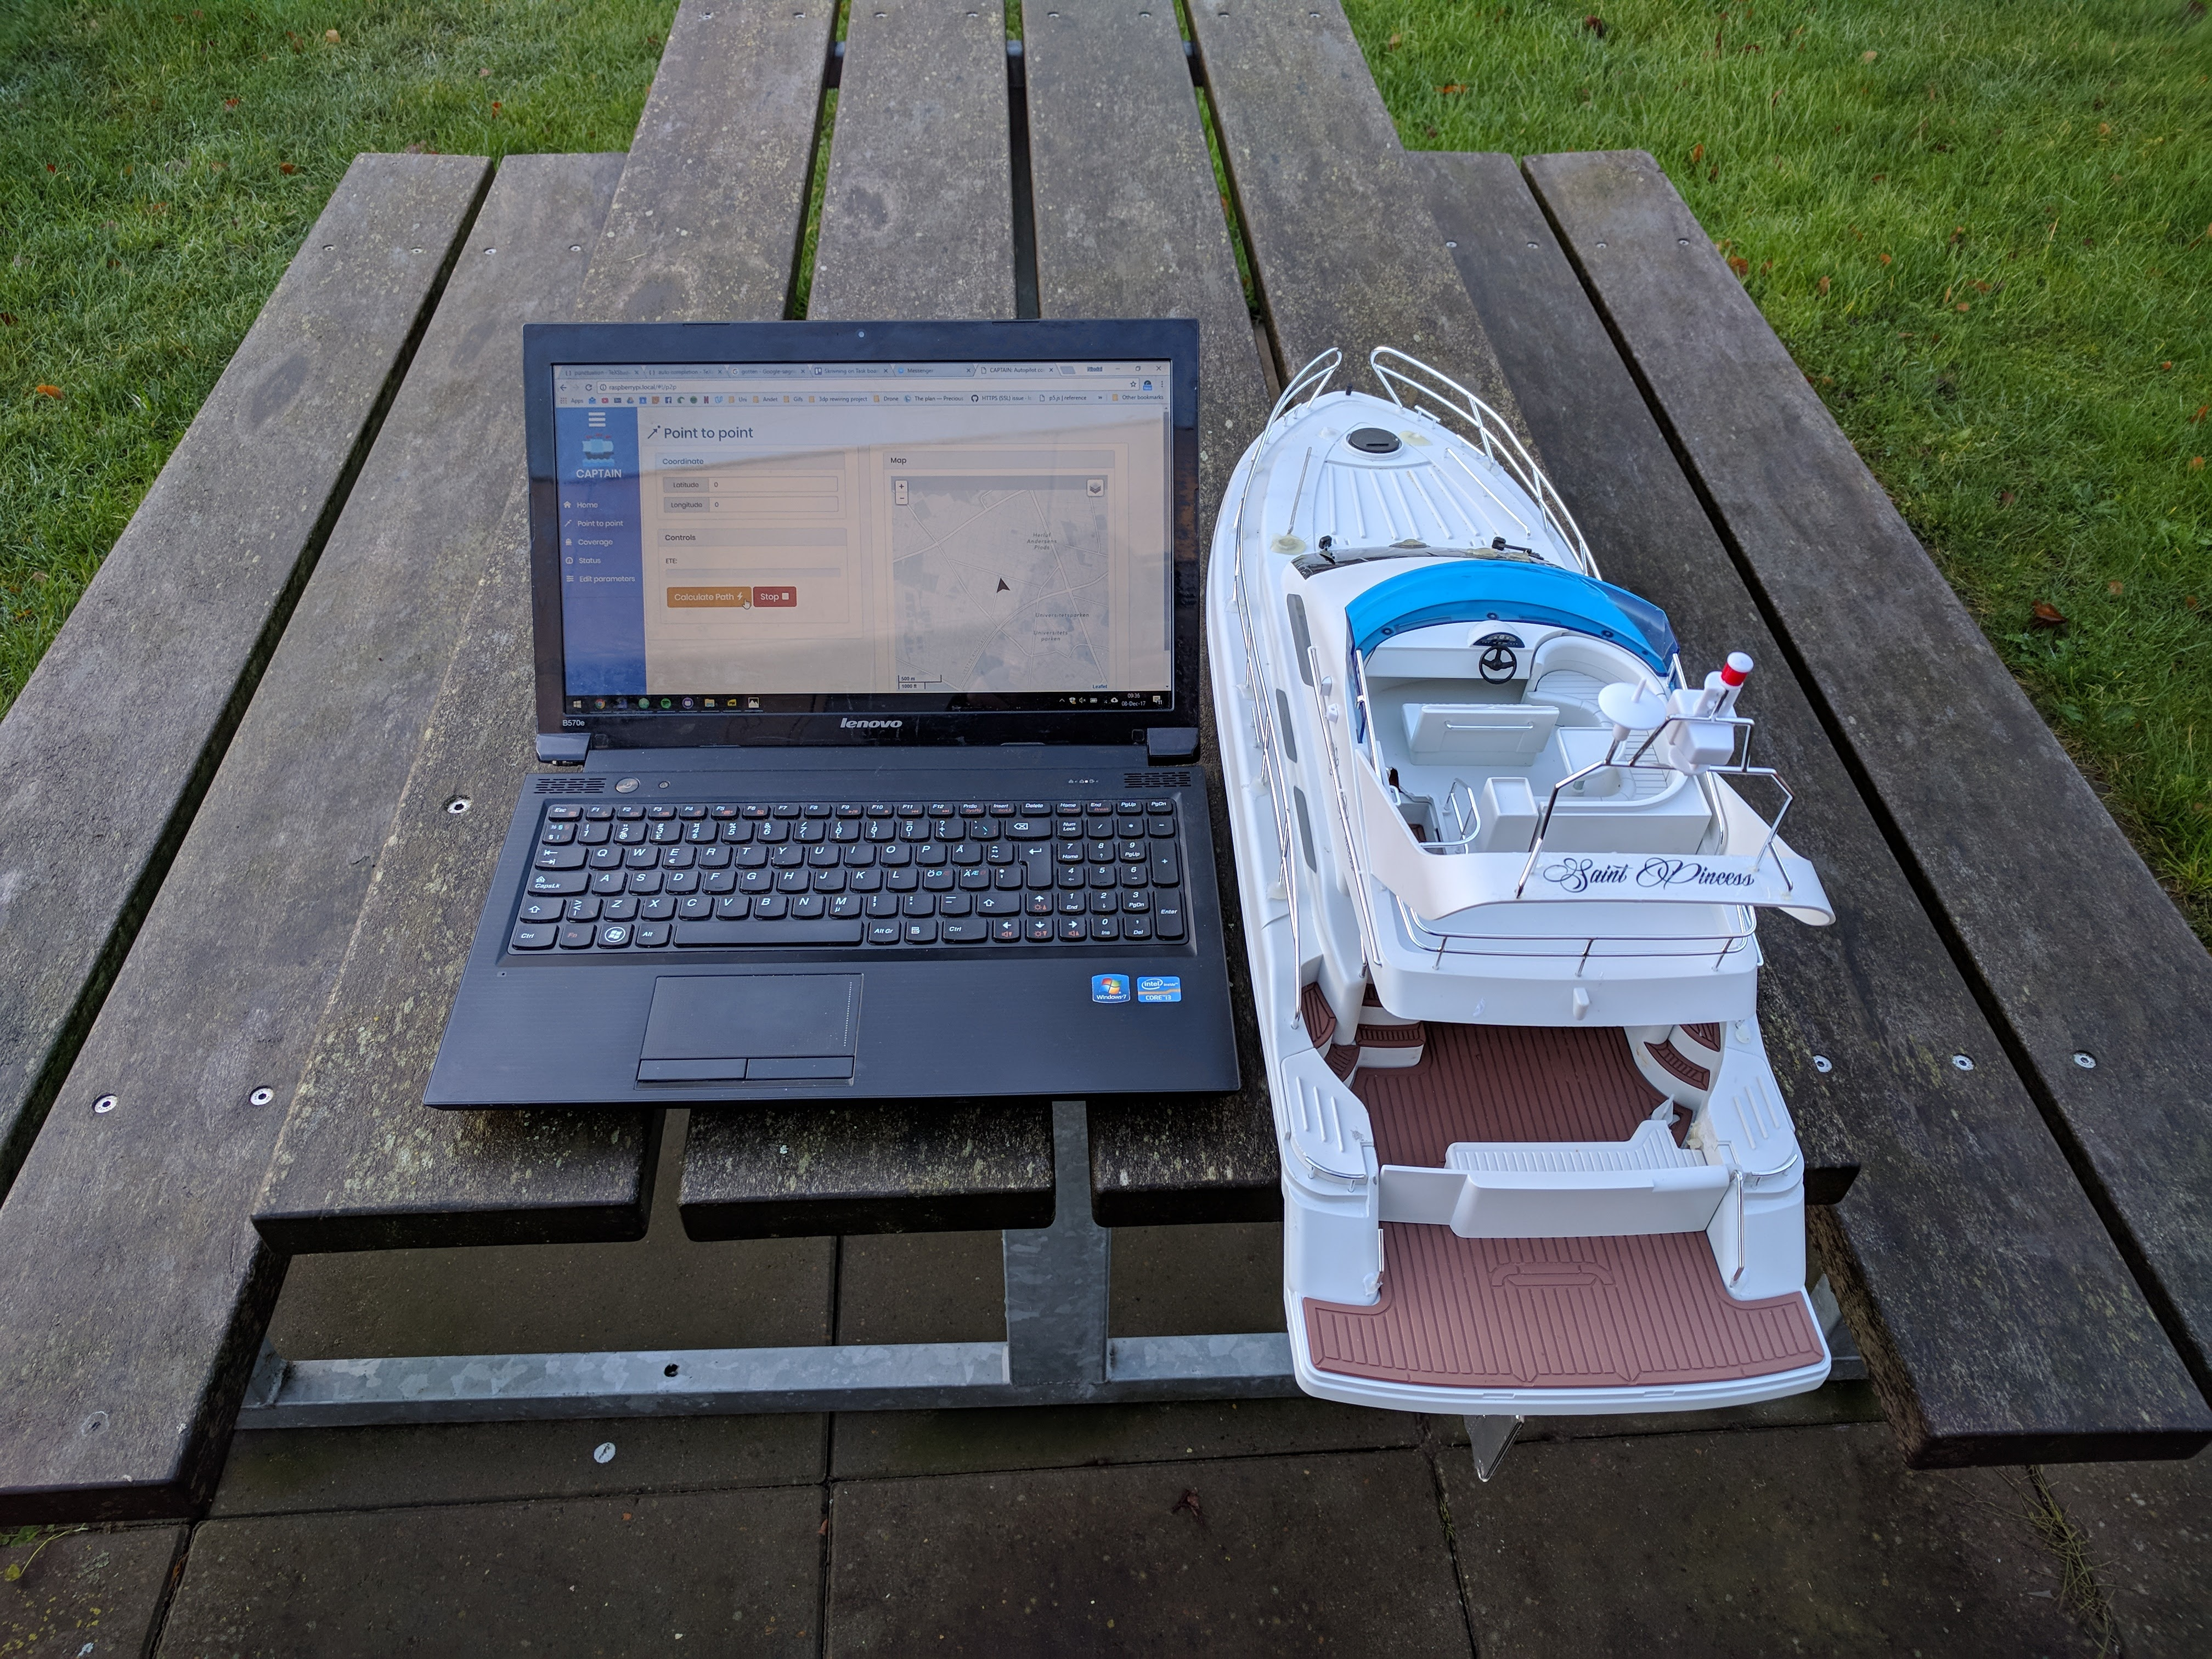
\includegraphics[width=0.7\linewidth]{Images/Integration/setup}
\caption{The setup used for integration testing}
\label{fig:integration_setup}
\end{figure}


\section{GPS Receiver - Status page}
First off testing the status page, which is mostly a test of the GPS receiver integration. The boat is placed out side for about 30 seconds, this is to make sure that the GPS receiver has fix. When fix is gained, the status page should display a fix of 1. There should also be some satellites connected, and the horizontal dilution of precision, should be as small as possible. As it can be seen in figure~\ref{fig:integration_statuspage}, the GPS receiver data is outputted correctly to the website user interface. Also it can be seen that the last message was got with in 10 seconds, so the data is not completely out of date. One thing to keep in mind is that there may be a offset in time on the boat and on the client computer.

\begin{figure}[H]
\centering
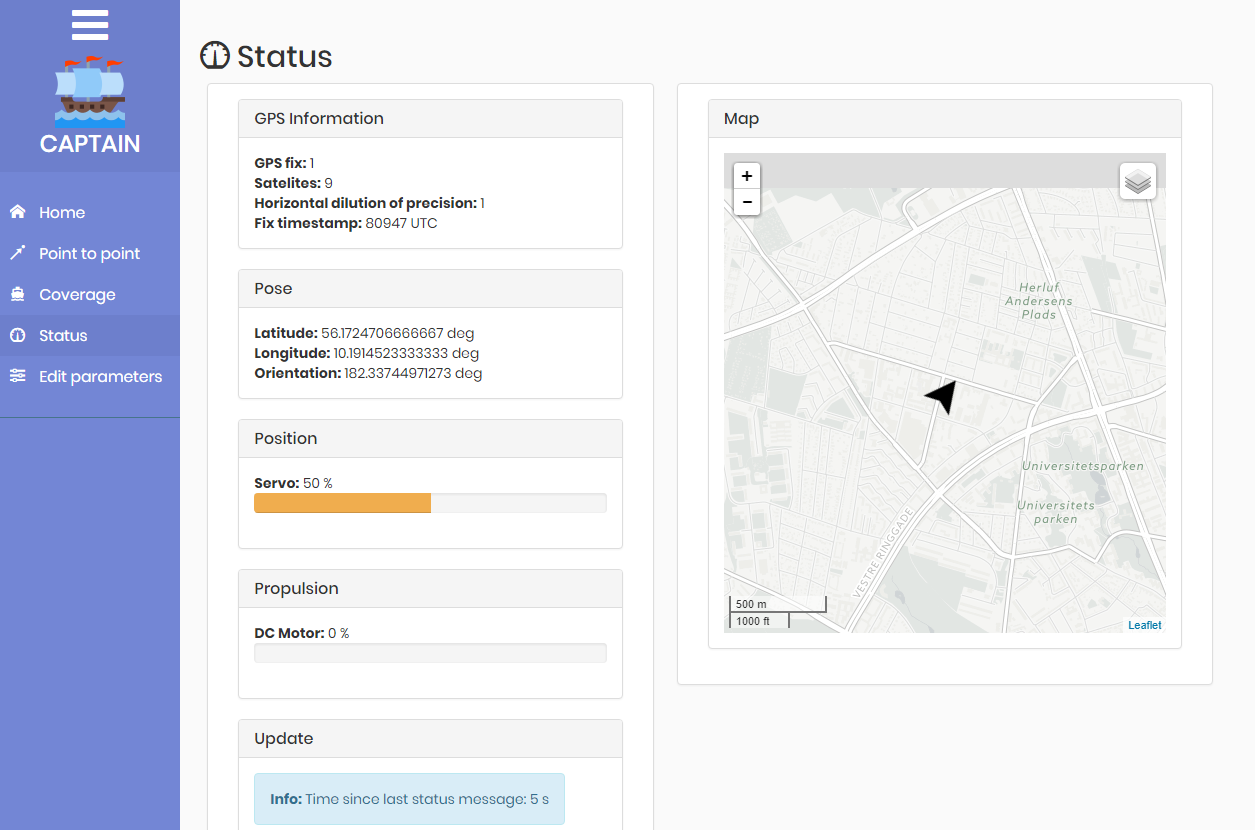
\includegraphics[width=0.9\linewidth]{Images/Integration/Status_page}
\caption{A view of the status page from the integration test}
\label{fig:integration_statuspage}
\end{figure}


\section{Motor, Servo, Point to point page, Coverage}
To test the integration of the motor and servo with the code base, the easiest way is to use the point to point page. A point was chosen on the map, and the calculate button was pressed. After a short while the map updated with a blue line from the boat position to the target. An example of this can be seen in figure~\ref{fig:pointtopoint}. In the example the boat has moved a bit and it can be seen that a green line is also displayed showing the progress.

\begin{figure}[H]
\centering
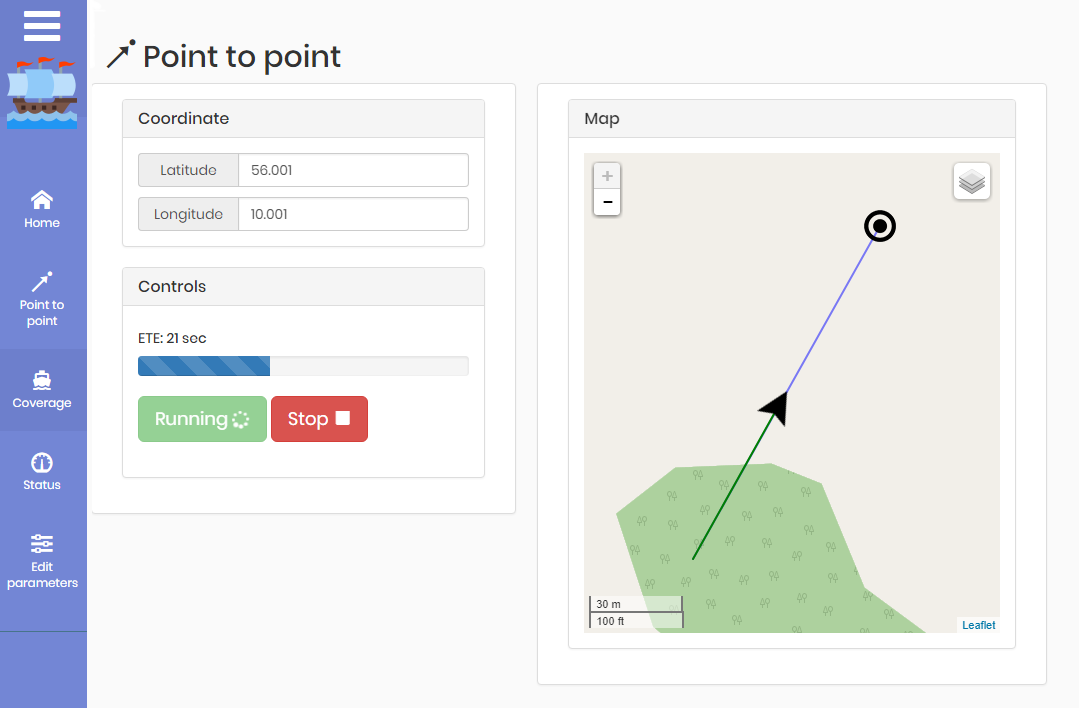
\includegraphics[width=0.9\linewidth]{Images/Integration/point_to_point}
\caption{A example of the point to point page like it was used in the integration test}
\label{fig:pointtopoint}
\end{figure}

When the Run button was pressed, the rudder turned to face the direction the boat wanted to go. An also the motor slowly turned up to speed. This can somewhat be seen in figure~\ref{fig:integration}.

\begin{figure}[H]
\centering
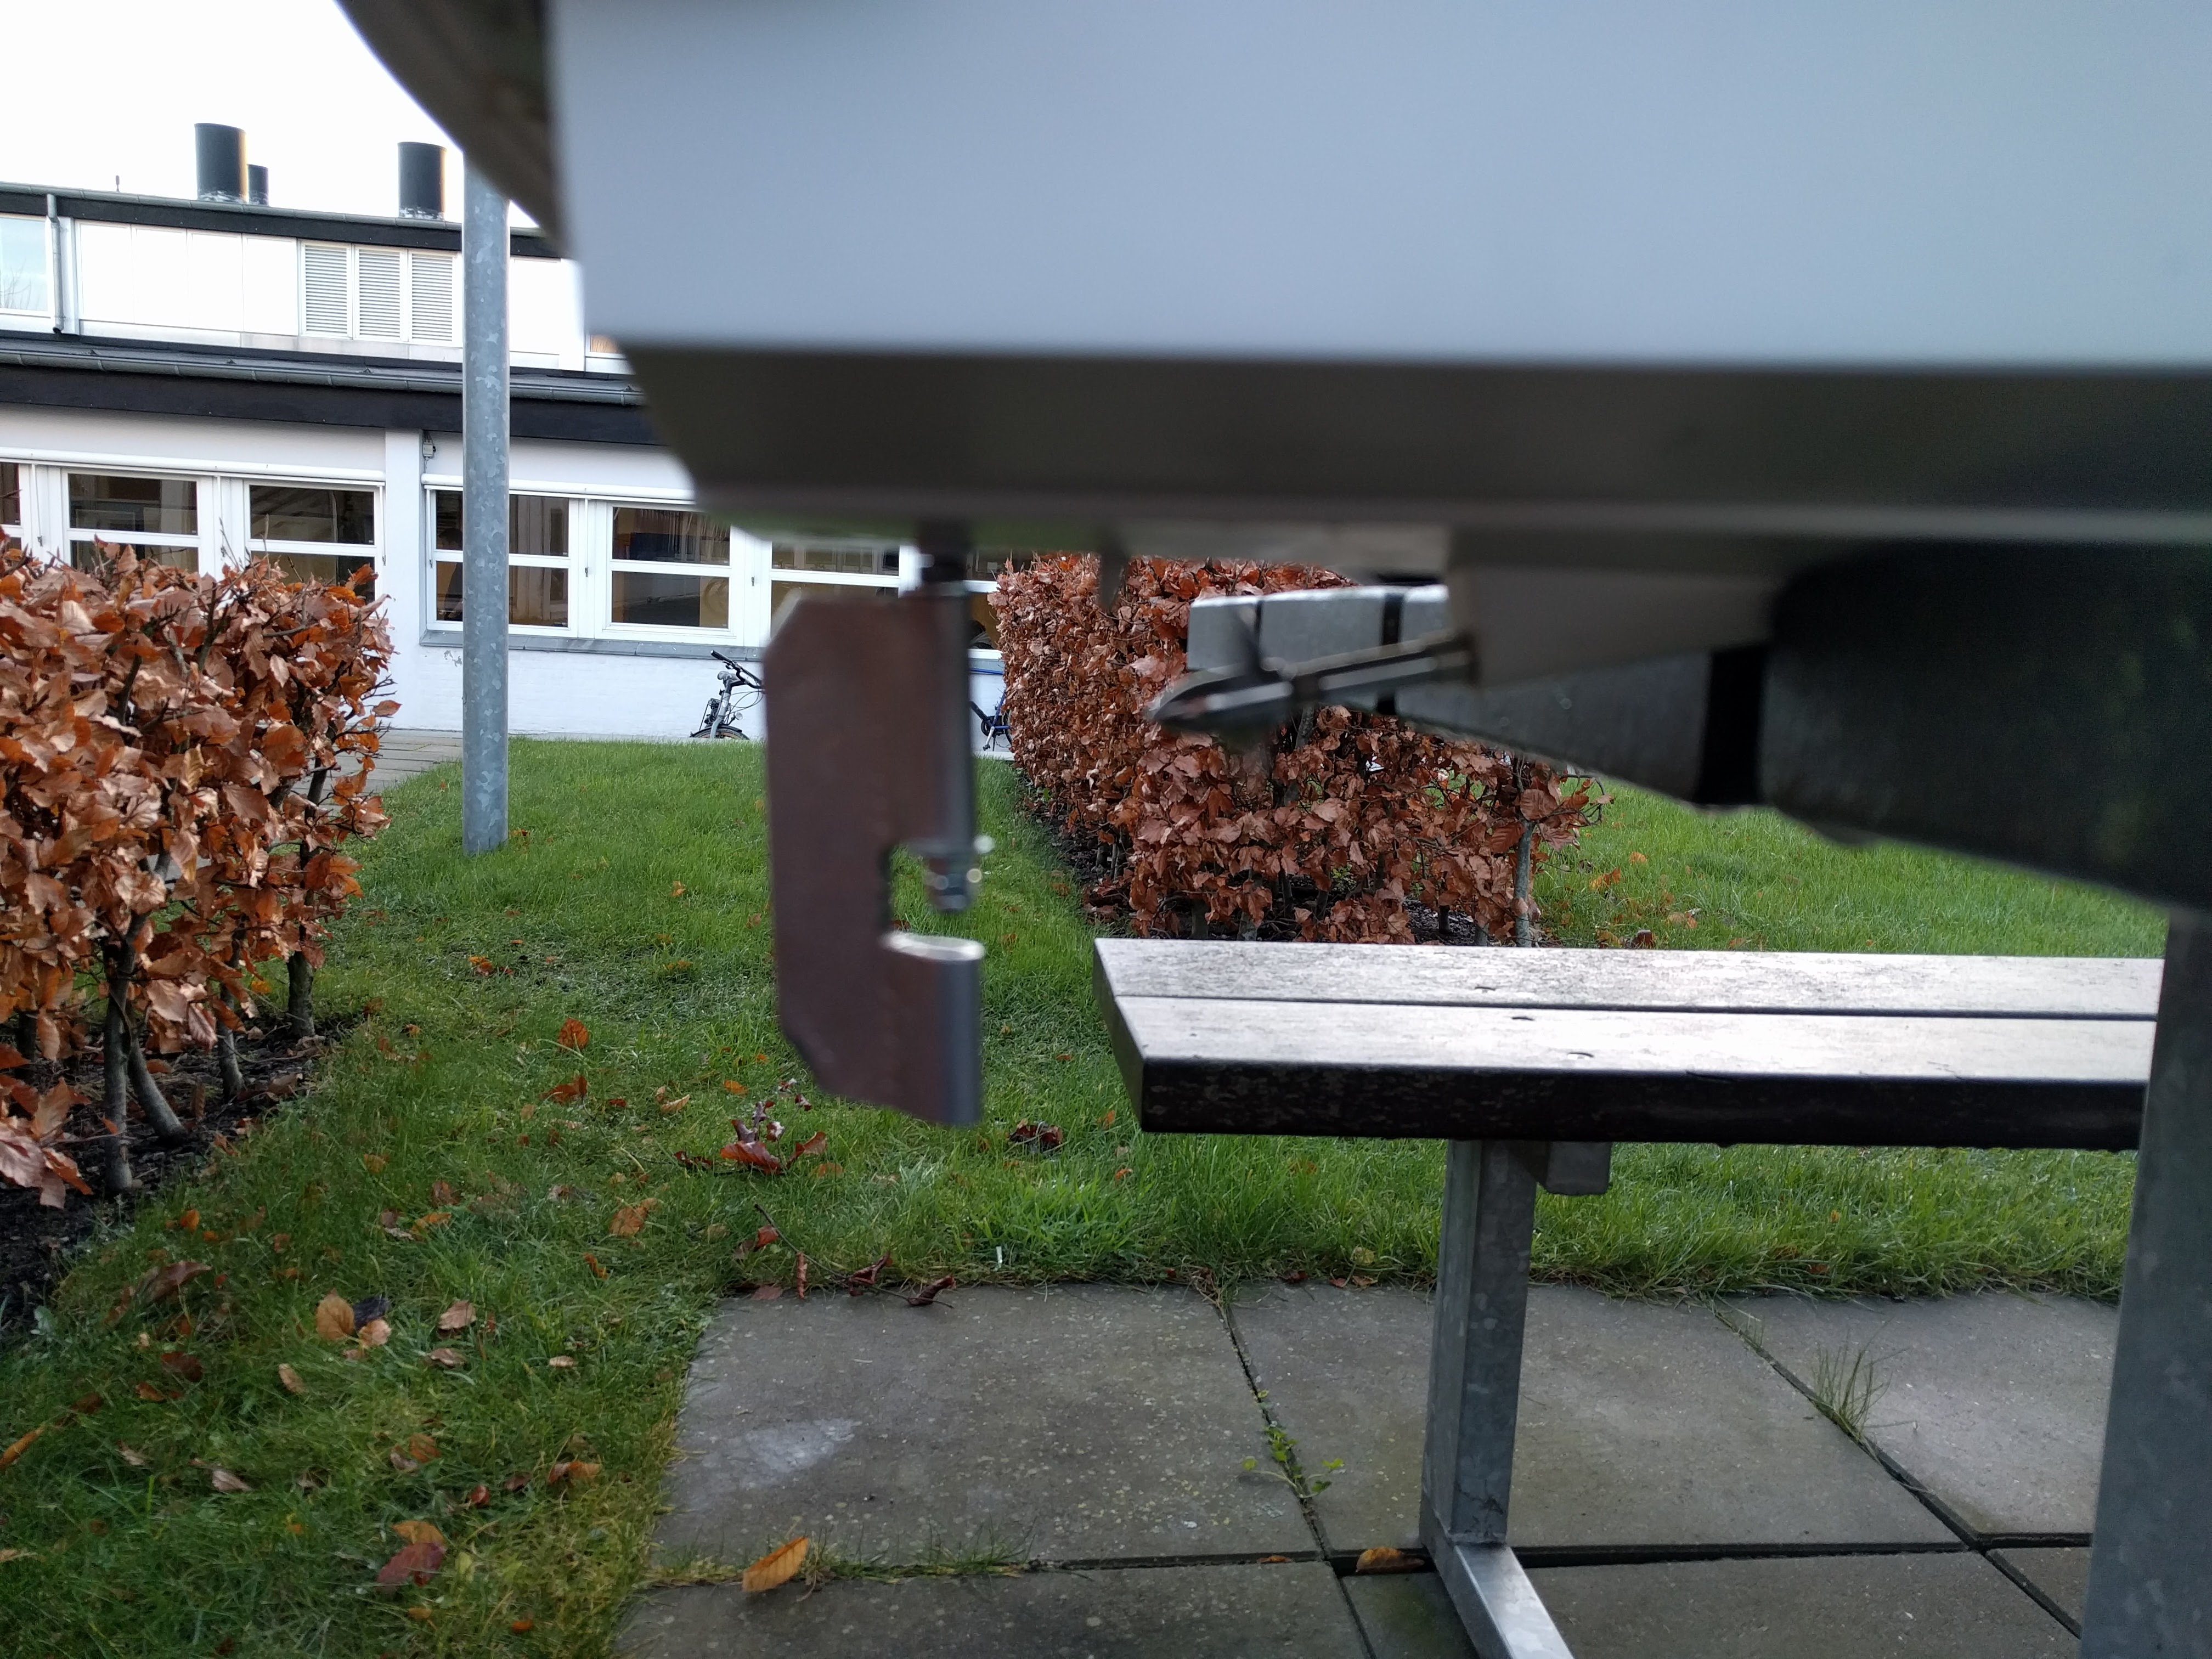
\includegraphics[width=0.7\linewidth]{Images/Integration/IMG_20171208_093712}
\caption{The motor rotating and the rudder being turned away from the camera}
\label{fig:integration_motor}
\end{figure}

The same test was conducted with the coverage page. In this case when the calculate button was pressed, a more complicated path was displayed on the website, just like in figure~\ref{fig:integration_coverage}. When the run button is pressed the motor begins running and the rudder adjusts. 

\begin{figure}[h]
\centering
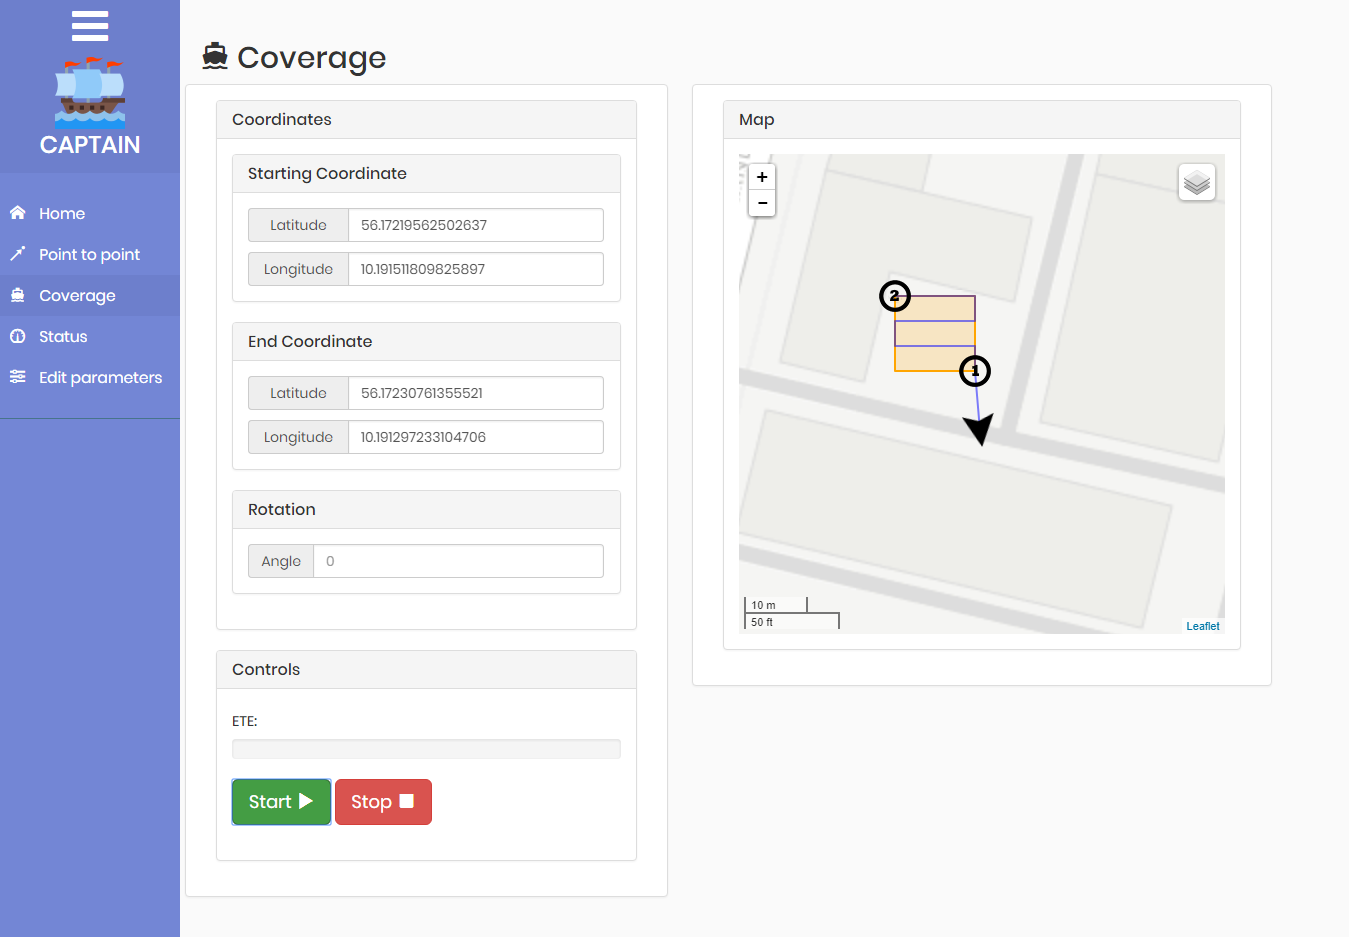
\includegraphics[width=0.9\linewidth]{Images/Integration/integration_coverage}
\caption{A path calculated by the boat to cover the selected area}
\label{fig:integration_coverage}
\end{figure}
 
When the boat had been through the entire path, the motor was stopped and the rudder was reset to the center. On the display the ETE reads "Arrived at target".1








